\chapter{CNN Architectures}

\section{Introduction}

This portion of the course provides a high-level overview on the history and evolution of convolutional neural networks, providing information on each advancement. This document will cover very brief summaries, it is advised to consult the slides for more reading.


\section{The CNN data}
\textbf{ImageNet Large Scale Visual Recognition Challenge (ILSVRC)}
\begin{itemize}
    \item The standard benchmark for comparing recognition systems (CNNs in this case)
    \item An annual competition since 2010, with 1.2 million images across 1000 classes
\end{itemize}

\section{CNN models}
\subsubsection{1989-1998  LeNet by Yann LeCun et all.}
\begin{itemize}
    \item 2 conv layers, 2 pooling layers, 2 FC layers, 60k parameters
    \item  \texttt{INPUT $\rightarrow$ CONV $\rightarrow$ SIGMOID $\rightarrow$ POOL $\rightarrow$ CONV $\rightarrow$ SIGMOID $\rightarrow$ POOL $\rightarrow$ FC $\rightarrow$ SIGMOID $\rightarrow$ FC}

    \item 99\% accuracy on MNIST
\end{itemize}

\subsubsection{2012 AlexNet by Alex Krizhevsky et al.}
\begin{itemize}
    \item Used LeNet with more data and GPUs.
    \item Increased from 2 to 5 conv layers, + 1 FC layer(now 3 layers) , each followed by ReLU instead of tanh, the activation function is 6 times faster
    \item Dropout 0.5 for FC layers instead of L2 regularisation. Training time doubled as a result
    \item 2 pooling layers to reduce netwok size
    \item 62.3M parameters, with conv layers representing 6\% of all parameters and 95\% of the total computation
    \item Top-5 error rate of 15.3\% on ImageNet at time of release
\end{itemize}

\subsubsection{2014 VGG by Karen Simonyan et al.}
\begin{itemize}
    \item Based on AlexNet, but replaced large filters in first two layers with $3\times 3$ filters.
    \item Use multiple stacked smaller size kernels
    \item Increase the representational capacity of the ConvNet for the same number of parameters
    \item Double the channels, use ReLU to avoid saturation
    \item Same number of FC layers.
    \item 138M parameters
    \item Top-5 error rate of 7.3\% on ImageNet at time of release
    \item Note: at this rate, networks are getting deeper and deeper due to gaining more filters. There is a risk of saturation and degraded performance
\end{itemize}

\subsubsection{2014 GoogLeNet by Christian Szegedy et al.}
\begin{itemize}
    \item Utilised the inception block – filters with multiple sizes that operate on the same level to capture different scales of detail. Goes for a wider approach instead of a deep approach
    \item Auxiliary classifiers used during training: they are like a``mini cnn" with conv layers, activation functions, pooling layers, and fc layers, that provide intermediate outputs. They make predictions based on features available and are a form of providing intermediate layers, they help reduce the vanishing gradient problem, by providing additional gradients.
    \item Max pooling followed by $1\times 1$ convolution to reduce depth before the $ 3 \times 3$ and $5 \times 5$ convolutions
    \item Uses global average pooling instead of FC layers
    \item Version 2 uses factorised filters to help improve speed.
    \item Top-5 error rate of 6.67\% on ImageNet at time of release (V1)
    \item V4 achieved lowest of 5\%
\end{itemize}

\subsubsection{2015-2016 Residual NN (ResNet) by Kaiming He et al.}
\begin{itemize}
    \item Utilised identity mappings in layers to allow for stacking layers without reducing network performance.
    \begin{figure}[H]
        \centering
        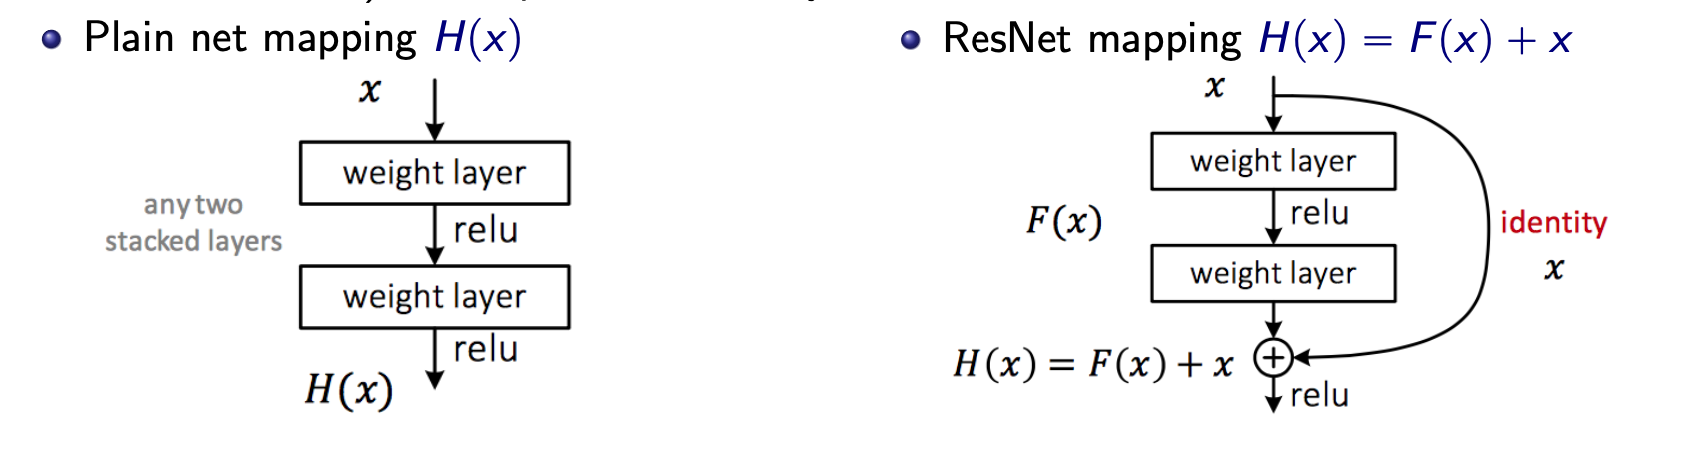
\includegraphics[width=0.7\linewidth]{img/resnet.png}
        
        
    \end{figure}
    \item The identity mapping allows the gradient to skip 1 or more layers using an ``identity shortcut connection"
    \item Skip connections allow the network to learn an identity function, which ensures that the higher layer will perform at least as well as the lower layer, and not worse.

    \item The identity skip connections enable the stacked layers to learn a residual mapping, which is essentially the difference between the desired underlying mapping and the identity function.
    
    \item The hypothesis is that it is easier to let the stacked layers learn (fit) this residual mapping than to learn the desired underlying mapping directly. 


    \item 2016 paper proposed 18, 50, 101, 152, 200 layer variants
    \item Most filters are $3 \times 3$ with global average pooling followed by the classification layer
    \item ResNet-200 achieved Top-5 error rate of 4.8\% on ImageNet at time of release, beating human performance
\end{itemize}

\subsubsection{2017 ResNeXt by Microsoft Research}
\begin{itemize}
    \item Combination of Google's Inception module and Kaiming He's skip connections
    \item Achieved Top-5 error rate of 4.4\% on ImageNet at time of release
\end{itemize}

\subsubsection{2017 DenseNet by Huang Gao et al.}
\begin{itemize}
    \item Allows skipping across multiple layers.
    \item ResNet: \( x_l = F_l(x_{l-1}) + x_{l-1} \)
    \item DenseNet: \( x_l = F_l([x_0, x_1, \ldots, x_{l-1}]) \)
    \item Achieves a stornger gradient flow, parameter and computational efficiency, and maintains low complexity features

\begin{figure}[H]
    \centering
    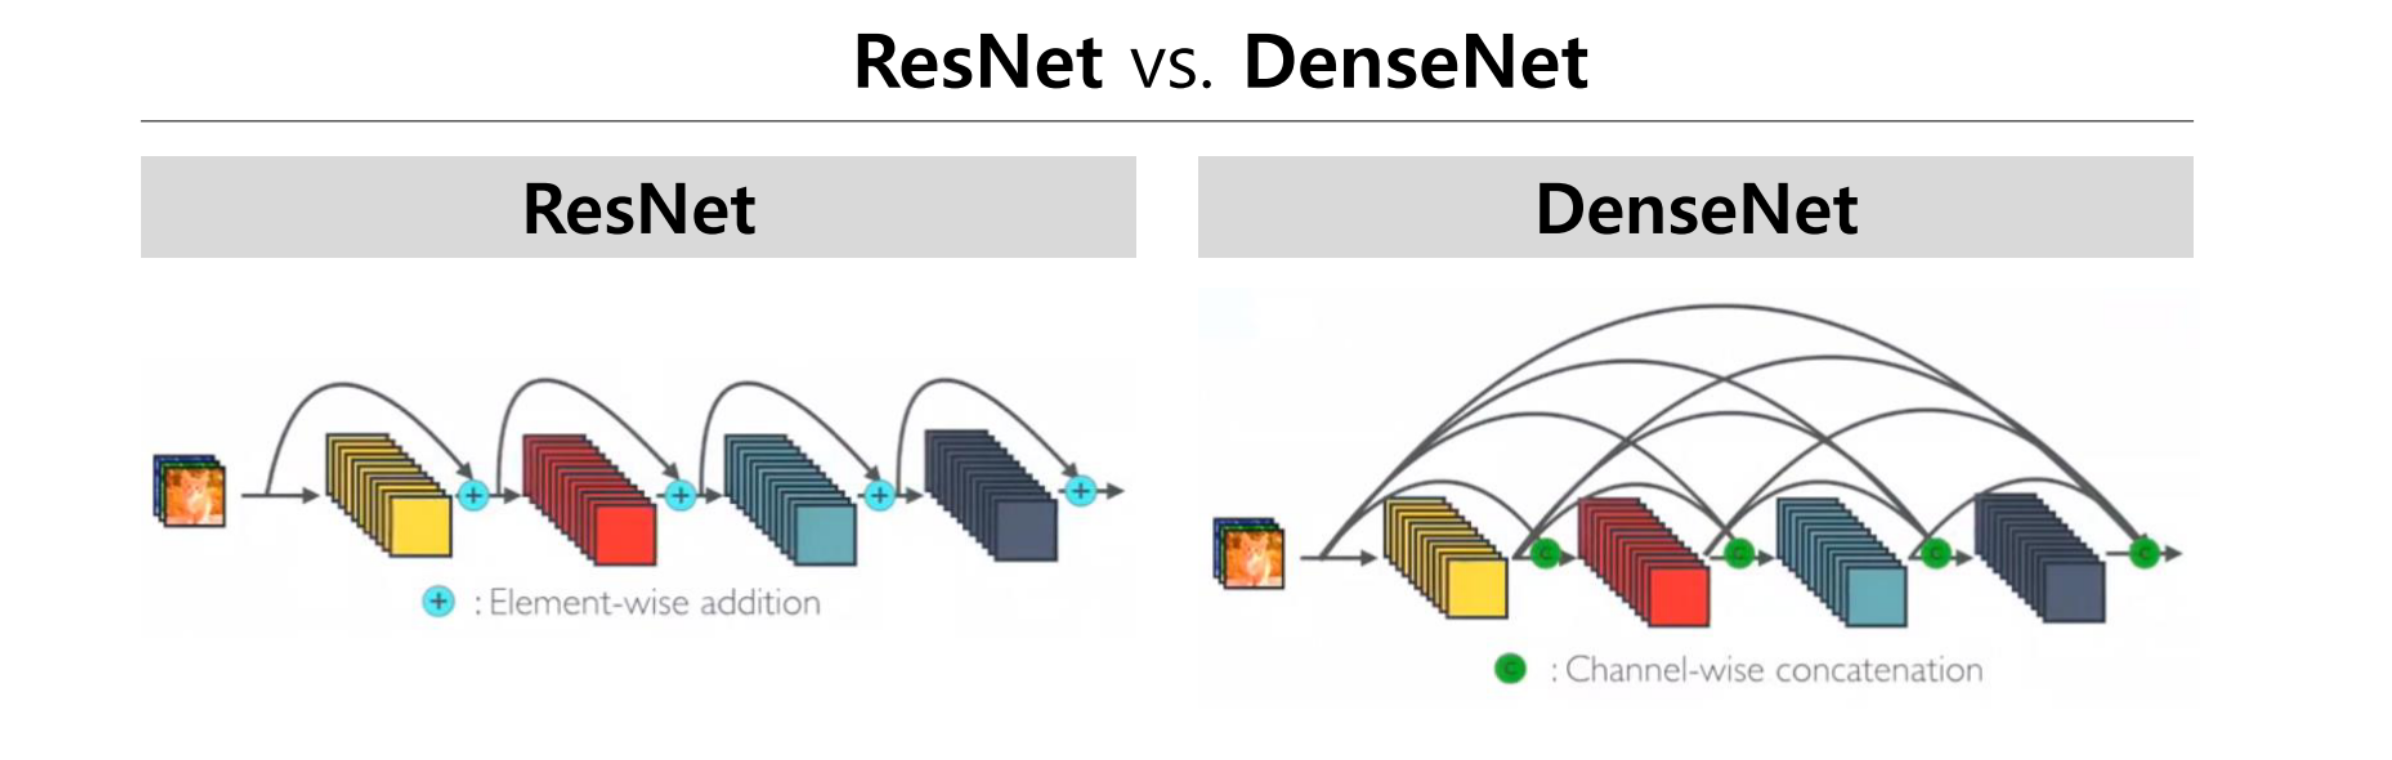
\includegraphics[width=0.75\linewidth]{img/densenet_resnet.png}
    
    
\end{figure}

\end{itemize}

\subsection{Performance Comparison}
\begin{figure}[H]
    \centering
    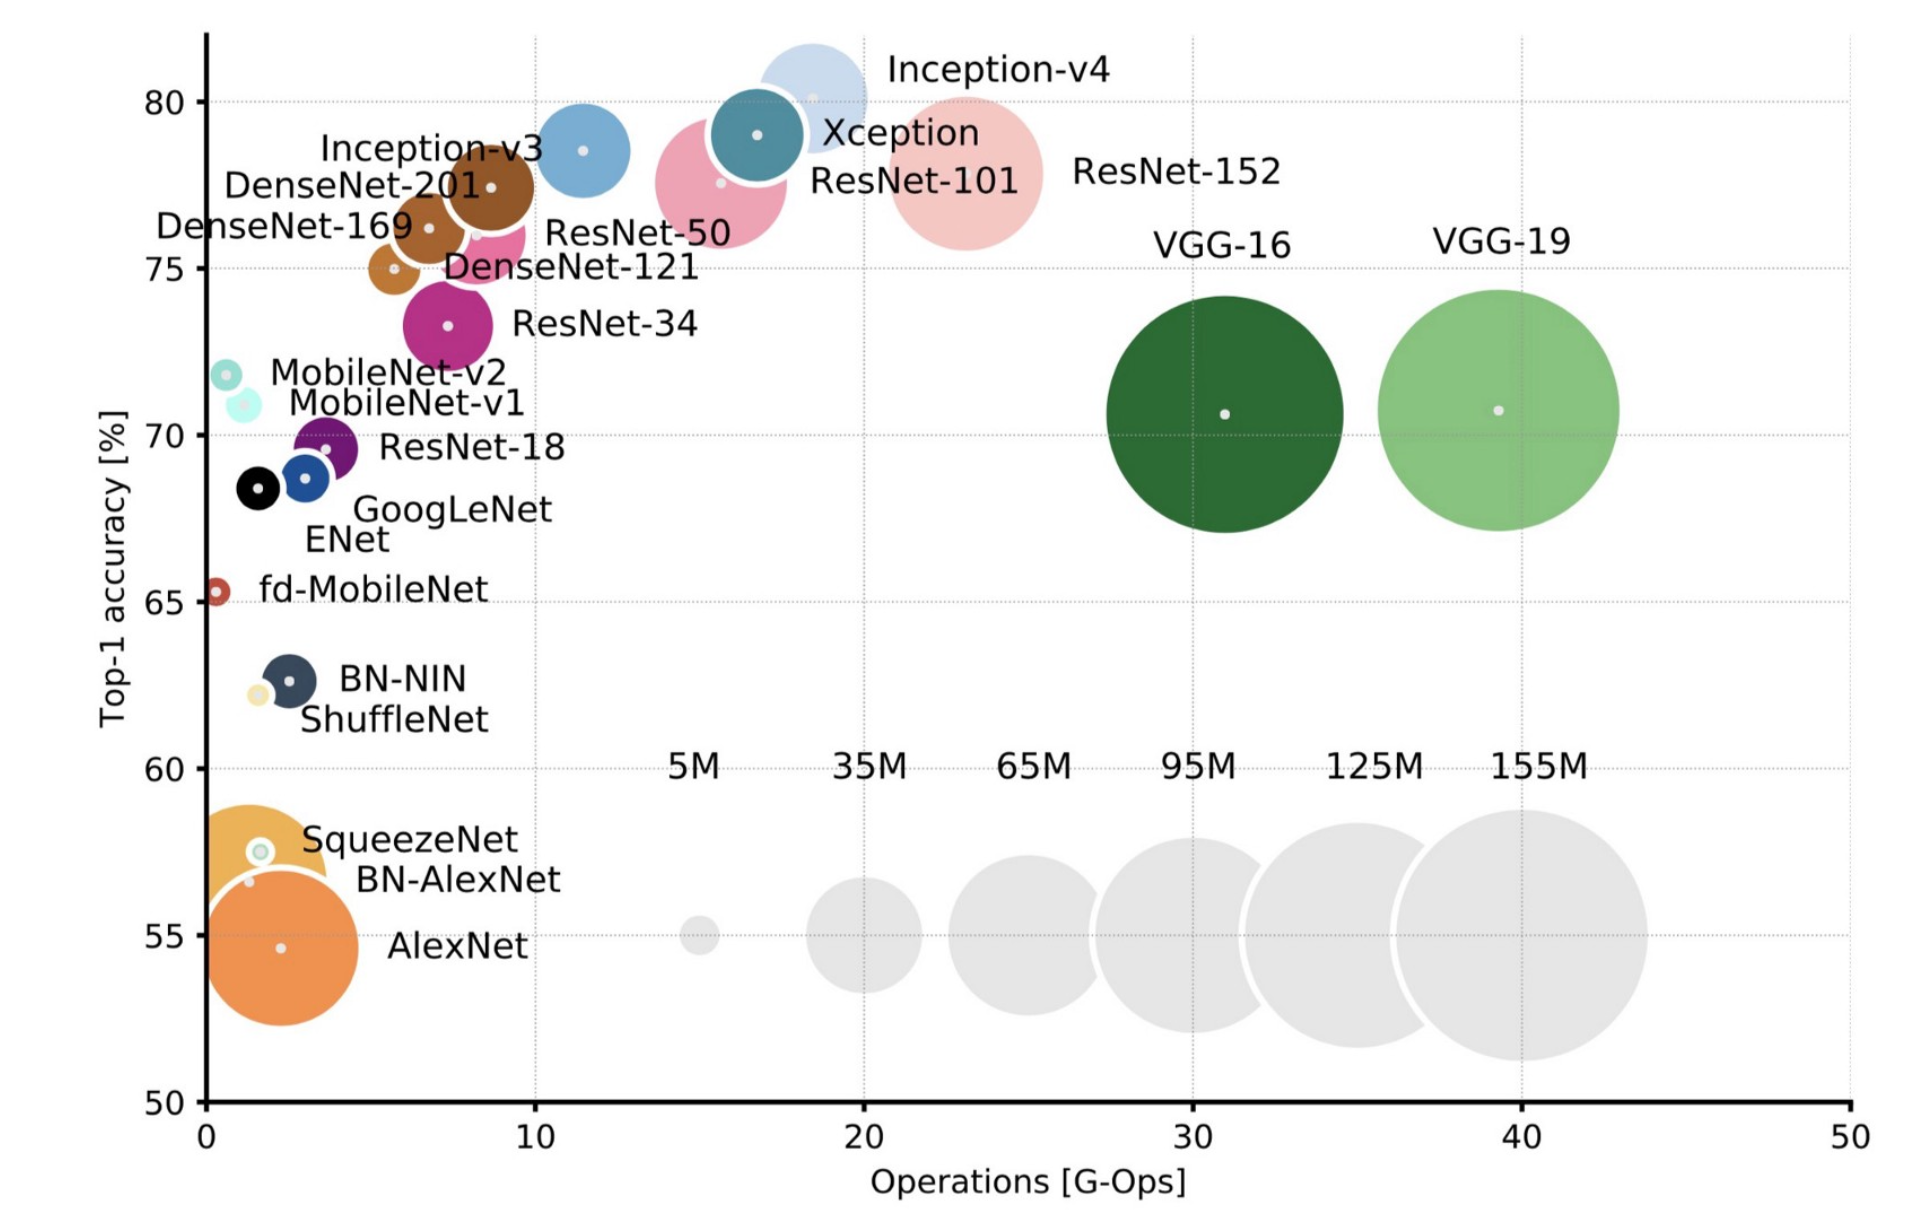
\includegraphics[width=0.8\linewidth]{img/cnn_performance.png}
    
    
\end{figure}

\subsection{CNN Encoder-Decoder Architecture}
\begin{itemize}
    \item Used for dense prediction tasks e.g. image segmentation, image enhancement, etc. Takes in an image and outputs and image.
    \item Typically, the encoder extracts feature maps by compressing input data into a condensed representation known as feature maps.
    \item The decoder's role is typically to take encoded feature maps and upsample/reconstruct them back to a desired input resolution (usually the original resolution), recovering spatial details that might have been compressed during encoding.
\end{itemize}

\subsubsection{Fully Convolutional Networks (FCN) by Long et al. (2015)}
\begin{itemize}
    \item Build FCNs that take input or arbitrary size and produce similarly sized output with efficient inference and learning
    \item Fully connected layers are viewed as convolutions with kernels that cover their entire input regions
    \item Upsampling done with backwards strided convolution

    \begin{figure}[H]
        \centering
        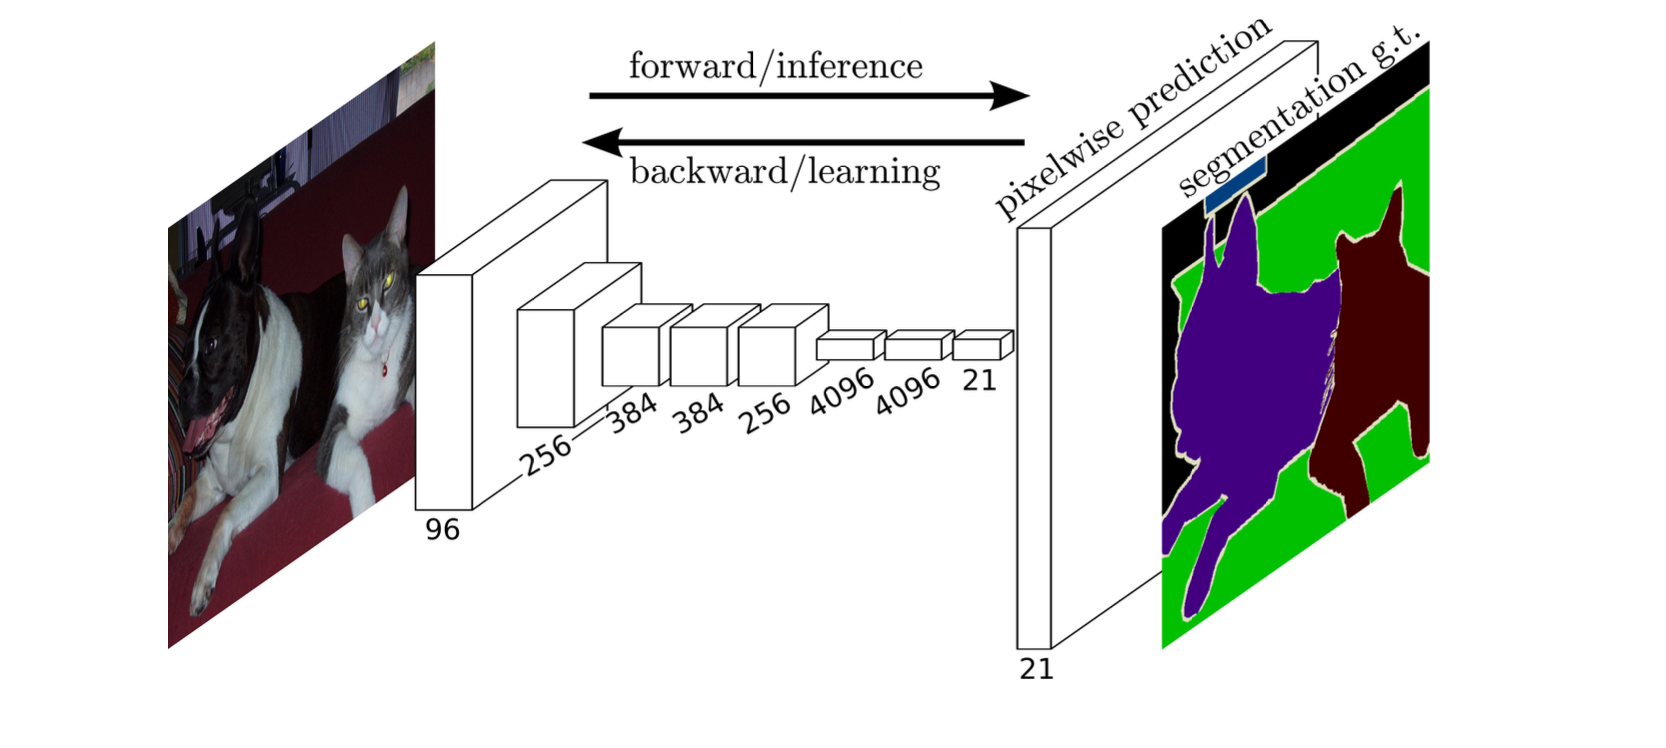
\includegraphics[width=0.75\linewidth]{img/FCN.png}
        
        
    \end{figure}
    
\end{itemize}

\subsubsection{U-Net by Ronneberger et al. (2015}
\begin{itemize}
    \item U-shaped architecture with skip connections and multi-scale feature maps
    \item Slightly more symmetrical than the FCN
    \begin{figure}[H]
        \centering
        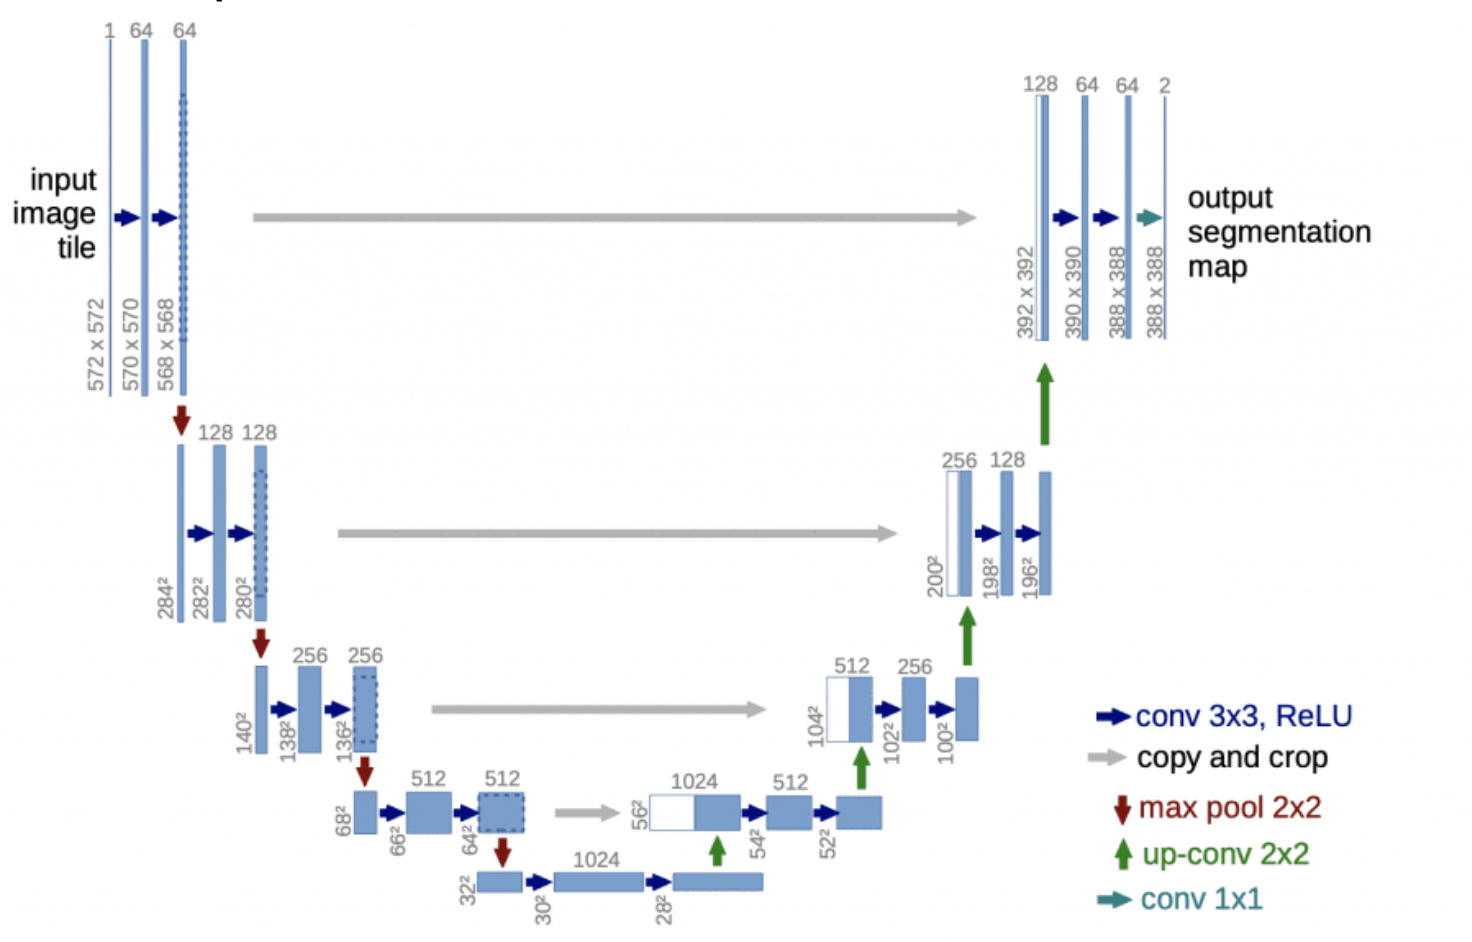
\includegraphics[width=0.5\linewidth]{img/u_net.png}
        
        
    \end{figure}
\end{itemize}

\subsubsection{CNN Siamese Networks}
\begin{itemize}
    \item Two networks in parallel trying to discern the transformation of an image given a before-after example
    \item L2 loss compares output features
    \item Shared FC layers possibly merge the output of two streams
    \begin{figure}[H]
        \centering
        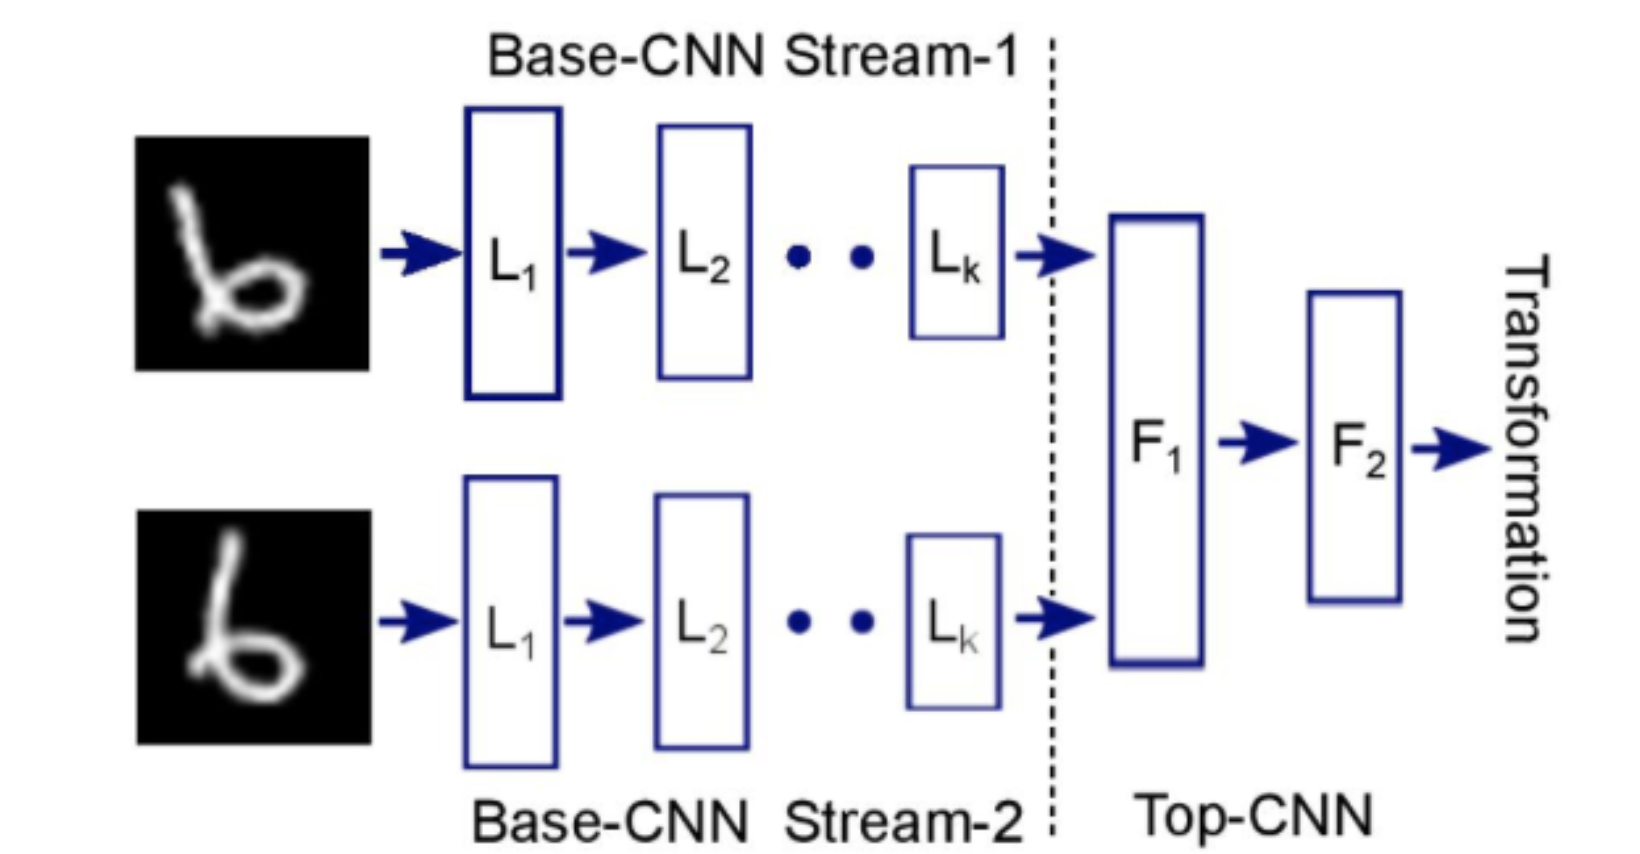
\includegraphics[width=0.75\linewidth]{img/siamese.png}
        
        
    \end{figure}
\end{itemize}

\subsubsection{Multitask Learning}
\begin{itemize}
\item Multi-task CNNs handle multiple learning tasks concurrently
\item An example could be classifying a type of animal, but also trying to localise it, determining its location with a bounding box.
\item They utilise shared layers to capture features common to all tasks, which can lead to better performance than learning separate models.
\item Task-specific layers are used on top of the shared layers to learn features unique to each task.
\item These networks can be more parameter-efficient and require less computational resources than separate models for each task. They often result in improved learning of features due to the regularising effect of jointly learning related tasks.
\end{itemize}

\begin{figure}
    \centering
    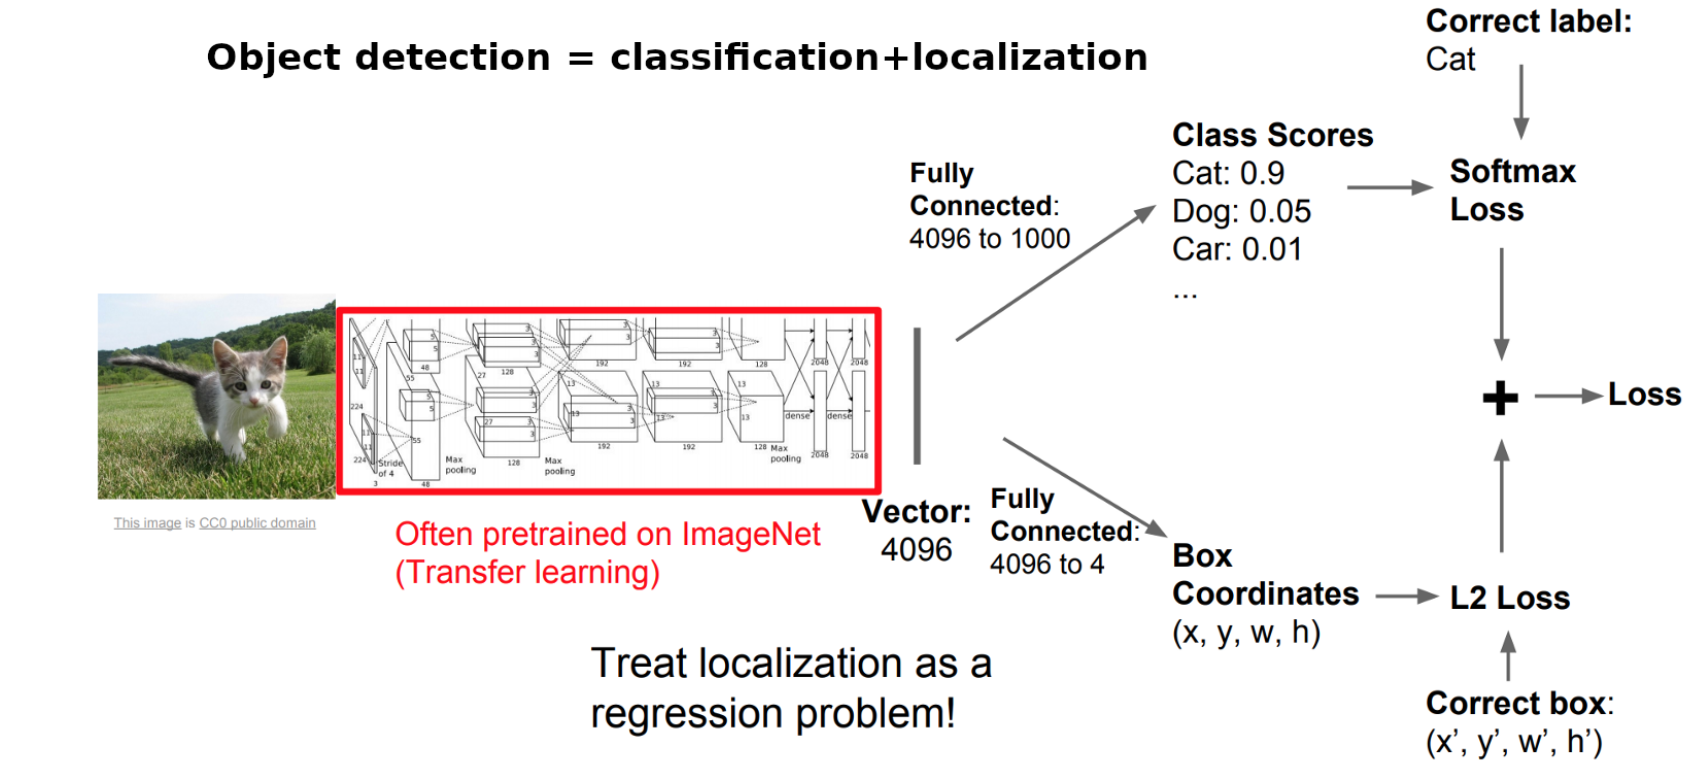
\includegraphics[width=0.75\linewidth]{img/multitask.png}
    
    
\end{figure}